\section{How to publish a repo?}

There are several ways to create a repository on \textsf{GitHub}, but here we will explain the two most common: starting from scratch, and starting with a previously initialized local Git repository.

\subsection{From scratch}

The easiest way to create a repository is by starting from the website. Once you have your account\footnote{Please, if you don't have a \textsf{GitHub} account yet, \href{https://github.com/join}{join here}.}, you can follow the following steps in the \textsf{GitHub} webpage.

In the upper-right corner of any page, click on the plus $+$ sign to display the drop-down menu and then select \textsf{New Repository}; then a section will appear like the screenshot shown in Figure \ref{fig:Repo}.

\begin{figure} %[htp]
    \centering
    \begin{tikzpicture}
    \sbox0{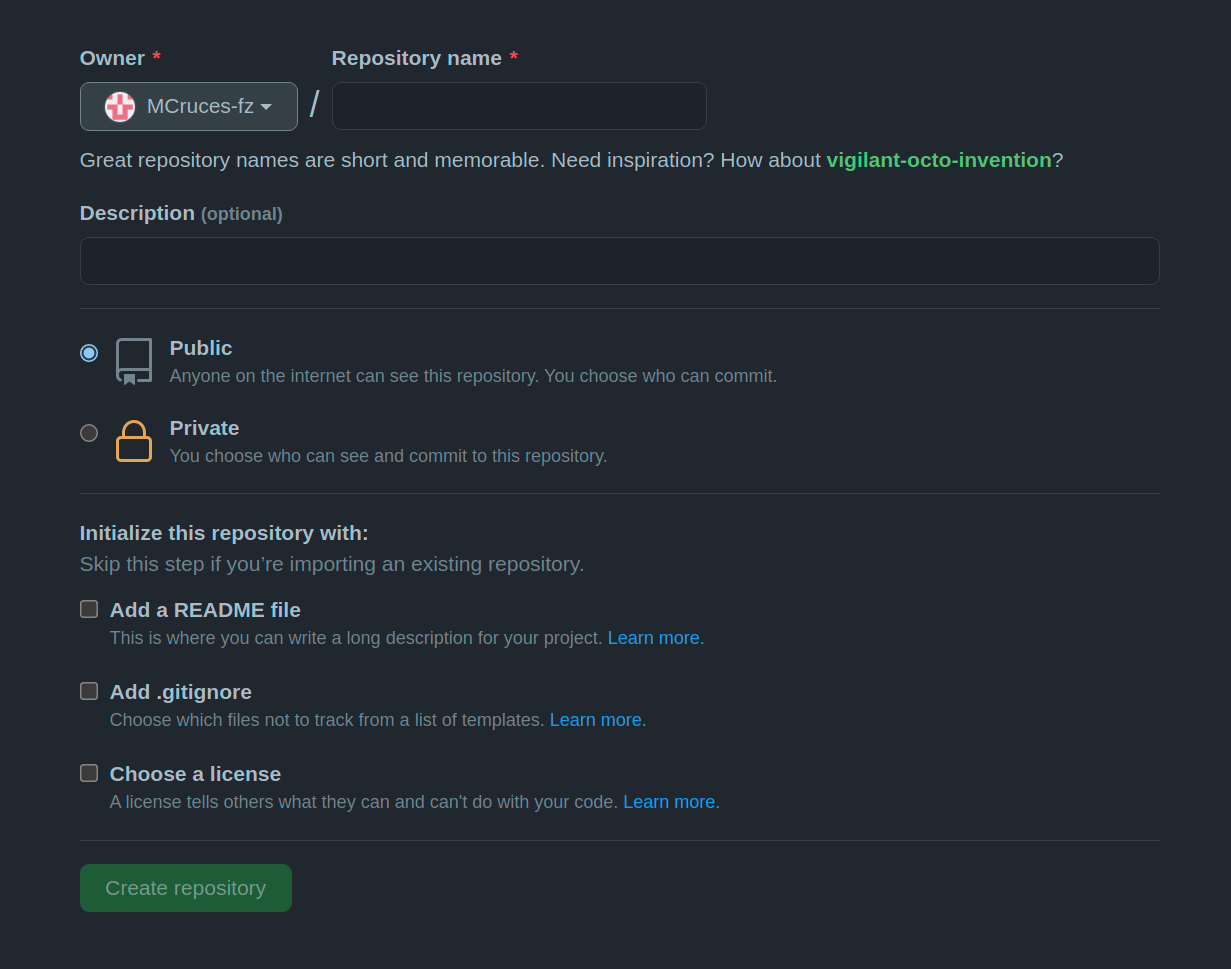
\includegraphics[width=\linewidth]{create_repo.png}}%
    \path[clip,rounded corners=10pt] (0,0) rectangle (\wd0,\ht0);
    \path (0.5\wd0,0.5\ht0) node[inner sep=0pt]{\usebox0};
    \end{tikzpicture}
    \caption{Example of creating a repository on \textsf{GitHub}.}
    \label{fig:Repo}
\end{figure}

Below the \textsf{Owner} drop-down menu you can choose your own user, or a group to which you belong. As we all know, it is difficult for scientists to choose original names and that is why \textit{Octocat} always tries to inspire us with a ``short and memorable'' name for our repositories.

Writing a \textsf{Description} is always recommended, although optional. This will help the user understand the subject of the project before clicking to read the code.

As you can see, it is only mandatory to fill in these two fields: \textsf{Owner}\textcolor{red}{*} and \textsf{Repository name}\textcolor{red}{*}, but in terms of visibility there are only two options and one of them must be chosen. If we are trying to create a open-source repository, I think it goes without saying that we should choose the \textsf{Public} option.

\textsf{GitHub} helps us by giving us the option to automatically create a series of plain text documents:
\begin{itemize}
    \item \textit{README.md}: A \href{https://www.markdownguide.org/getting-started/}{markdown} file which will be displayed in your repository. Here you can write a more detailed description for your project.
    \item \textit{.gitignore}: This is a \textit{dotfile}\footnote{Those are hidden files in \textsf{Linux}.} where you can write which files not to track. Once you click on the checkbox, a drop-down menu will appear and you can choose a \textit{.gitignore} template\footnote{Of course, each type of project has a series of files that do not need to be shared, since they are generally compiled, executed...}.
    \item \textit{LICENSE}: Here you can choose a license for your repository, but we will see it in more detail in the next section.
\end{itemize}

Before clicking \textsf{Create repository}, you can change the default branch name to \texttt{master} instead of \texttt{main} \href{https://github.com/settings/repositories}{here}.

\subsection{From a local \textsf{Git} repo}

Maybe you have a local project and you want to publish it. If so, you can do it cleanly by following these steps.

First follow the steps written in previous section ``From scratch'', but stop once you had choosen the visibility of the repo. Don't add any files! as you can see, \textit{Octocat} suggests you skip that step if you're importing an existing repository, because when you push your files there will be merge conflicts (believe me you don't want that). Once this is done, you can \textsf{Create repository} and you will see some help commands.

Open your favorite terminal emulator and \texttt{cd} into the root directory of your project. Then, initialize a git local repository as follows

\begin{lstlisting}[style=shell]
cd /path/to/root/dir/
git init  # Initialize git repo (a directory .git/ appears)
git remote add origin https://github.com/<username>/<reponame>.git  # Add remote
vim .gitignore  # Edit a .gitignore if you want
git add --all  # Track all files except .gitignored
git commit -m "Mi first commit"  # Write a commit message 
git push -u origin master  # Push your new branch to GitHub
\end{lstlisting}


\subsection{Magit}

As is written in the \href{https://github.com/next-exp/IC/blob/master/CONTRIBUTING.md#use-a-higher-level-git-interface}{\textit{CONTRIBUTING.md}} of \href{https://github.com/next-exp/IC}{\textsf{next-exp/IC}} project:

\vspace{8pt}

{\Large \textit{``}}
\textit{Do yourself a favour, and use \href{https://magit.vc/}{magit} to interact with git: \href{https://magit.vc/quotes/}{it's the best git UI} on the planet. Even if you don't use or dislike Emacs, use magit, and think of Emacs as the GUI framework in which magit is written.}

\textit{You will enjoy and learn to understand git much more if you use magit.}

\textit{[Editor's note: Seriously, I tried to find something to recommend for those who don't use Emacs. It wasted a lot of my time, and I came to the conclusion that recommending anything else would be a waste of your time. Just use magit.]}

\textit{To make the magit experience even better, use \href{https://emacs-helm.github.io/helm/}{helm}.}
{\Large \textit{''}}

\vspace{8pt}

This tool is very useful to interact with git. The easiest GUI maybe is \textit{GitHub Desktop}, but it isn't powerful enough.

% \begin{figure} %[htp]
%     \centering
%     \begin{tikzpicture}
%     \sbox0{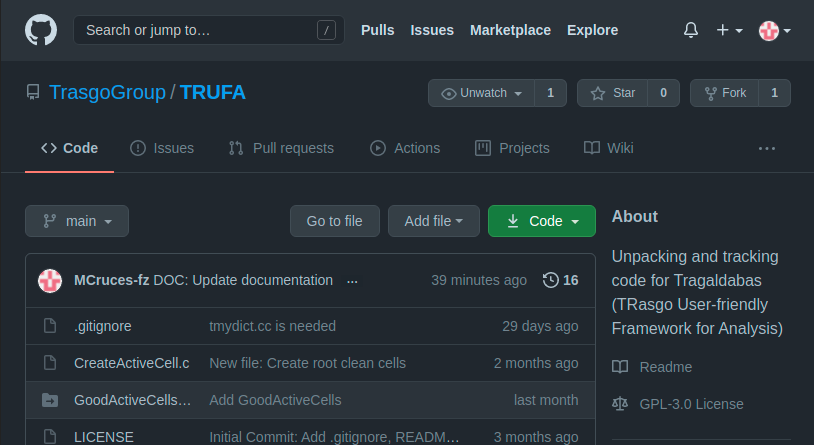
\includegraphics[width=\linewidth]{how_to_fork.png}}%
%     \path[clip,rounded corners=10pt] (0,0) rectangle (\wd0,\ht0);
%     \path (0.5\wd0,0.5\ht0) node[inner sep=0pt]{\usebox0};
%     \end{tikzpicture}
%     \caption{\textsf{Fork} button is in the top-right margin of the page.}
%     \label{fig:Fork}
% \end{figure}
